\begin{frame}
\frametitle{About This Work...}

\emph{Leveraging Spatio-Temporal Redundancy for RFID Data Cleansing}.~\cite{chen2010leveraging} \\
H.~Chen, W-S.~Ku, H.~W and M-T.~S.\\~\\

\begin{itemize}
  \item Published at \emph{SIGMOD' 2010}.
  \item Proposed a Bayesian inference based approach for cleaning RFID raw data.
  \item Desined an $n$-state detection model to capture the likelihood.
  \item Devised a Metropolis-Hastings sampler with Constraints (MH-C) to sample from the posterior.
\end{itemize}

\end{frame}

%------------------------------------------------

\begin{frame}
\frametitle{Motivation}

To take full advantage of:

\begin{itemize}
  \item duplicate readings (by multiple readers simultaneously or by a single reader over a period of time) of the same object are very common.
  \item prior knowledge about the readers and the environment (e.g., prior data distribution, false negative rates of readers) may help improve data quality and remove data anomalies.
  \item given constraints in target applications (e.g., the number of objects in a same location cannot exceed a given value).
\end{itemize}

\end{frame}

%------------------------------------------------

\begin{frame}
\frametitle{Data Redundancy: Spatial Redundancy}

\fsize{\textrm{The challenge is how to take advantage of redundancy while avoiding its undesirable effect in data cleansing.}}

\vspace{-10pt}
\begin{columns}[c]

  \column{0.5\textwidth}
  \begin{figure}[tb]
    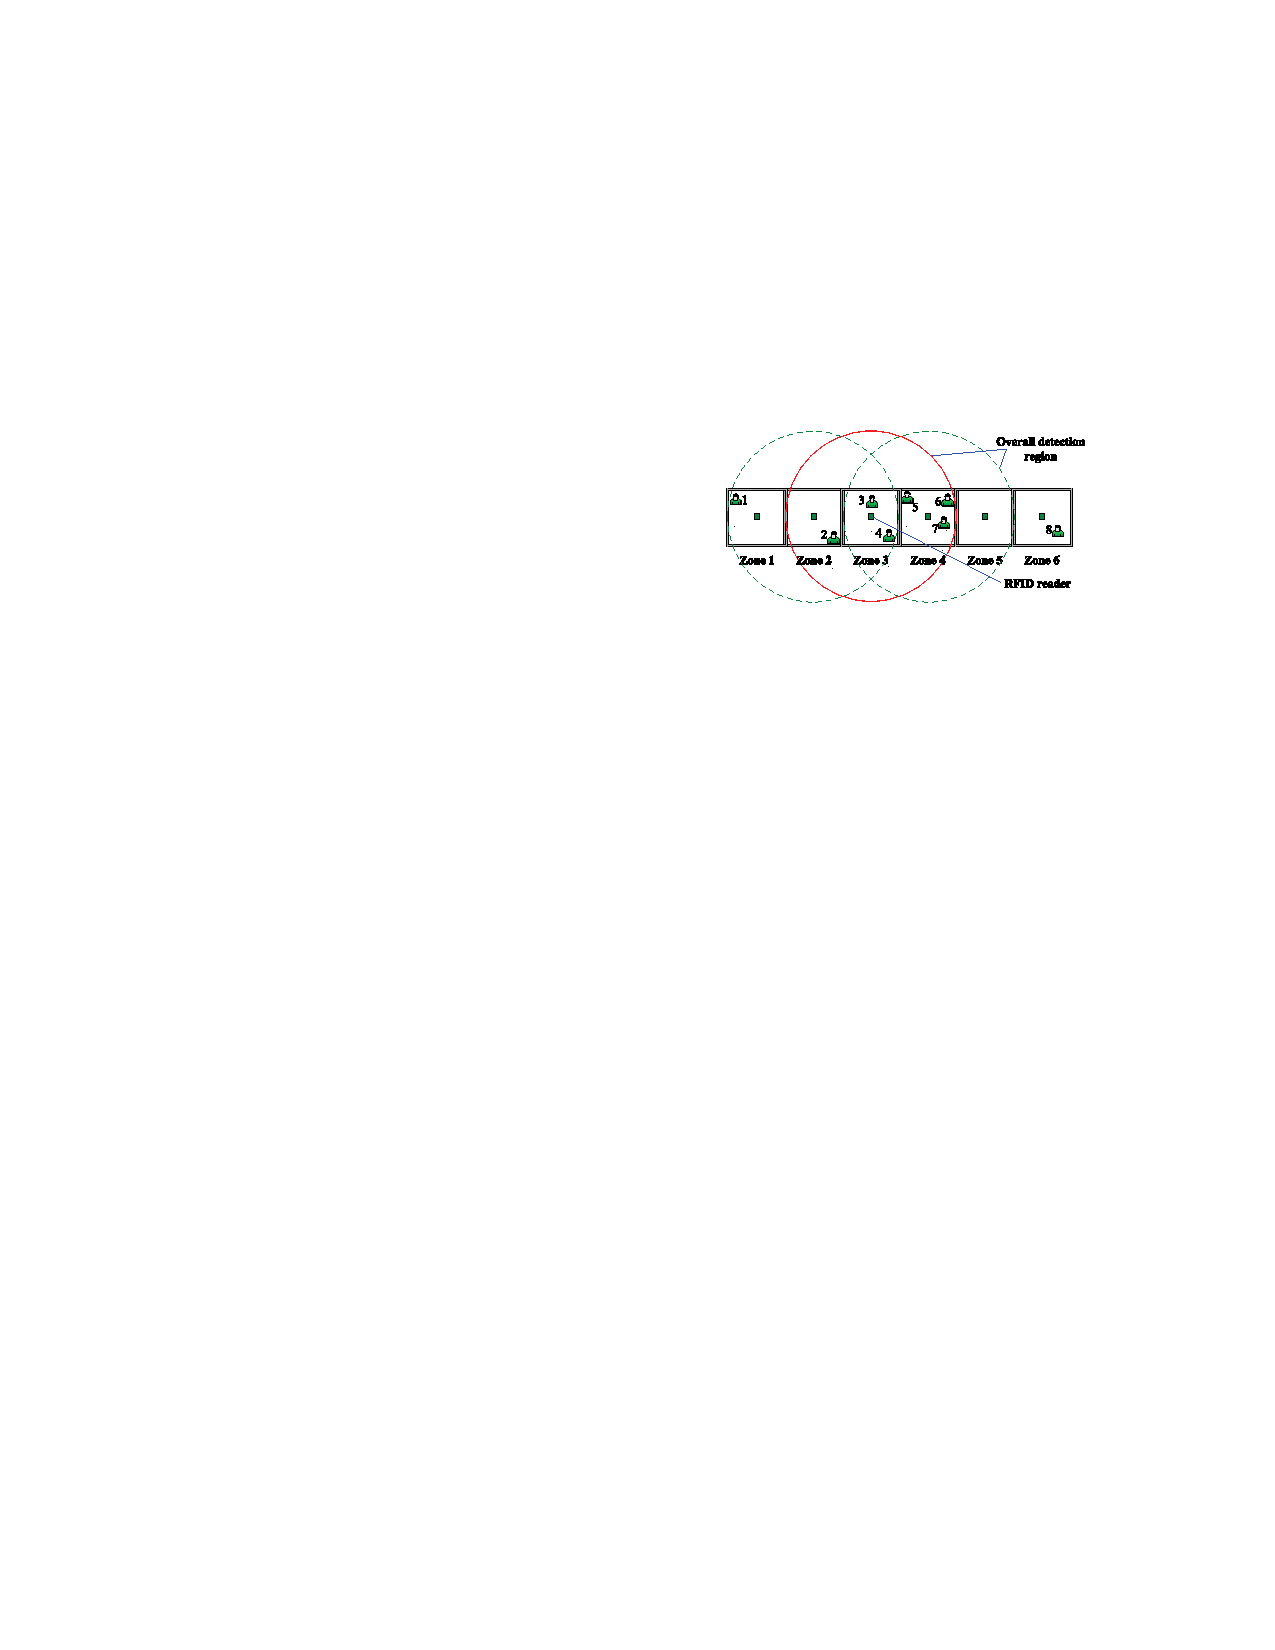
\includegraphics[width=\columnwidth]{figures/3-1/3-1-2.pdf}
  \end{figure}

  \begin{example}
    \ssize{
    \textrm{
    the target area is divided into 6 zones, an RFID reader is located in the center of each zone. Spatial overlap of readers' detection regions leads to duplicate readings, i.e., an object is in the detection regions of multiple readers.
    }}
  \end{example}

  \column{0.5\textwidth}
  \begin{figure}[tb]
    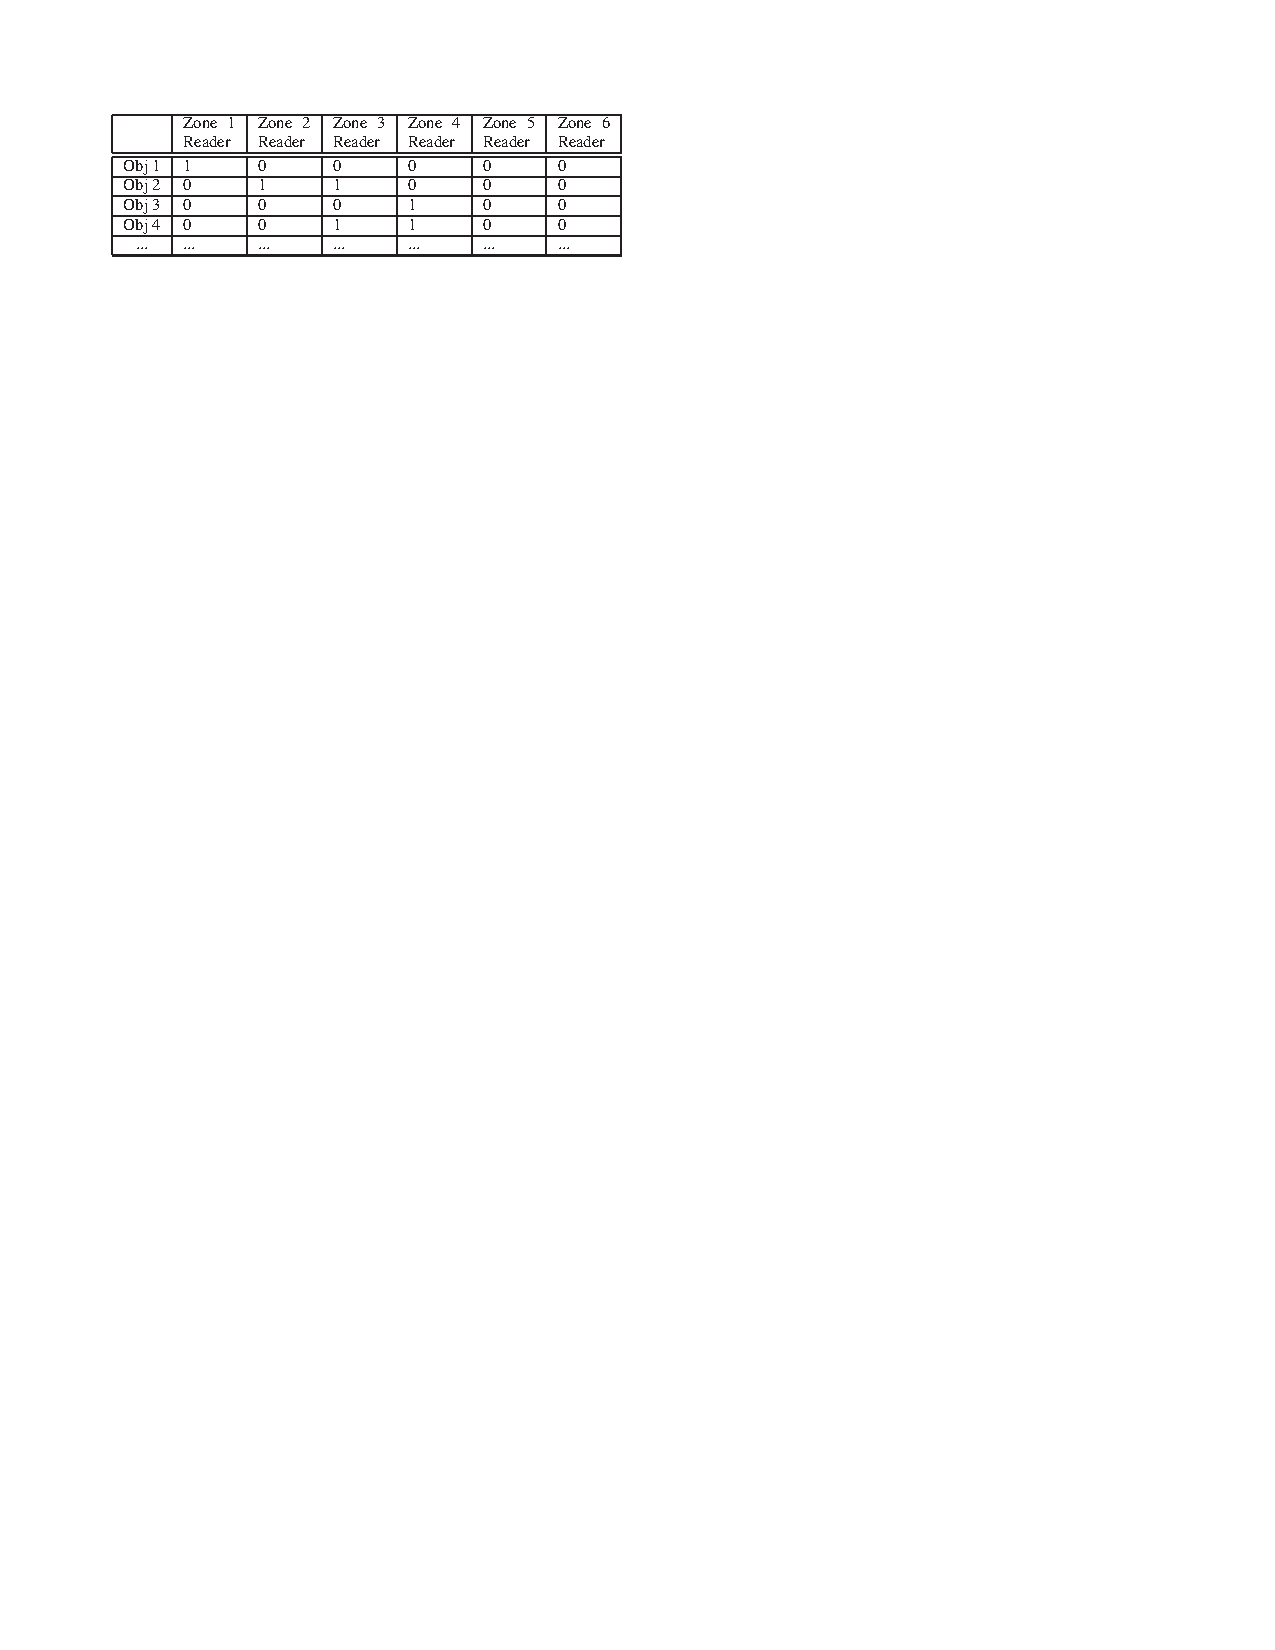
\includegraphics[width=\columnwidth]{figures/3-1/3-1-1.pdf}
  \end{figure}

  \ssize{
  The above table shows two effects of redundancy:
  \begin{enumerate}
    \item Object 2 is detected by both readers in Zone 2 and 3, at least one of the readings belongs to spatial redundancy.
    \item Object 3 is detected in Zone 4 only, however, it does not necessarily mean that the Object 3 is in Zone 4 for sure.
  \end{enumerate}
  }

\end{columns}

\end{frame}

%------------------------------------------------

\begin{frame}
\frametitle{Data Redundancy: Temporal Redundancy}

Many applications monitor the target area using a \emph{mobile reader} instead of employing multiple \emph{stationary readers}.\\~\\

Because the exact location of the mobile reader is always changing, the detection regions at different time points may overlap.\\~\\

\textbf{The temporal redundancy problem can be reduced to the spatial redundancy problem:} by treating the same reader at different time points as different readers.

\end{frame}

%------------------------------------------------

\begin{frame}
\frametitle{Prior Knowledge}

As false negatives and false positives abound in raw RFID readings, in order to revoer the true information, the data cleasing system should take prior knowledge into account.\\~\\

For example, the detection areas of readers in Zone 2 and 3 have significant overlapping, the positioning of the reader in Zone 4 makes it more likely to detect objects in Zone 3 than objects in Zone 5, or the reader in Zone 3 has high false negative rate.

\end{frame}
